% -- Generated using the code: resting_clocks_fitted_single_fig(0, 6, 0.5, 0.3)



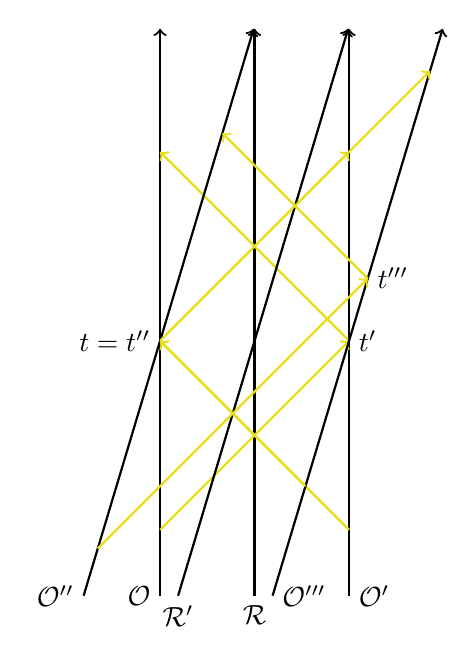
\begin{tikzpicture}[scale=1.2]
	% First resting observers
	
	%			% Draw lines of observers
	%		    \draw[->, thick] (-0.19065934065934065, 0) -- (-0.19065934065934065, 6);
	%		    \draw[->, thick] (2.007142857142857, 0) -- (2.007142857142857, 6);
	%		    \draw[->, thick] (0.8999999999999999, 0) -- (0.8999999999999999, 6);
	%		
	%		    % Draw trajectories of light
	%		    \draw[->, thick, black!10!yellow] (-0.19065934065934065, 0.5) -- (2.007142857142857, 2.697802197802198);
	%		    \draw[->, thick, black!10!yellow] (2.007142857142857, 2.697802197802198) -- (-0.19065934065934065, 4.895604395604396);
	%		    \draw[->, thick, black!10!yellow] (2.007142857142857, 0.5) -- (-0.19065934065934065, 2.697802197802198);
	%		    \draw[->, thick, black!10!yellow] (-0.19065934065934065, 2.697802197802198) -- (2.007142857142857, 4.895604395604396);
	%		
	%		    % Make labels
	%		    \draw (-0.19065934065934065, 0) node[left] {$\mathcal{O}''$};
	%		    \draw (2.007142857142857, 2.697802197802198) node[right] {$t'$};
	%		    \draw (2.007142857142857, 0) node[right] {$\mathcal{O}'''$};
	%		    \draw (-0.19065934065934065, 2.697802197802198) node[left] {$t = t''$};
	%		    \draw (0.8999999999999999, 0) node[below] {$\mathcal{R}'$};
	
	
	
	% Version 2 of code, different goal now: same x-distances between resting, moving ones -> then we can really see asynchrony
	
	
	% Draw lines of observers
	\draw[->, thick] (-0.19065934065934065, 0) -- (-0.19065934065934065, 6);
	\draw[->, thick] (1.8093406593406594, 0) -- (1.8093406593406594, 6);
	\draw[->, thick] (0.8093406593406594, 0) -- (0.8093406593406594, 6);
	
	% Draw trajectories of light
	\draw[->, thick, black!10!yellow] (-0.19065934065934065, 0.697802197802198) -- (1.8093406593406594, 2.697802197802198);
	\draw[->, thick, black!10!yellow] (1.8093406593406594, 2.697802197802198) -- (-0.19065934065934065, 4.697802197802198);
	\draw[->, thick, black!10!yellow] (1.8093406593406594, 0.697802197802198) -- (-0.19065934065934065, 2.697802197802198);
	\draw[->, thick, black!10!yellow] (-0.19065934065934065, 2.697802197802198) -- (1.8093406593406594, 4.697802197802198);
	
	% Make labels
	\draw (-0.19065934065934065, 0) node[left] {$\mathcal{O}$};
	\draw (1.8093406593406594, 2.697802197802198) node[right] {$t'$};
	\draw (1.8093406593406594, 0) node[right] {$\mathcal{O}'$};
	\draw (-0.19065934065934065, 2.697802197802198) node[left] {$t = t''$};
	\draw (0.8093406593406594, 0) node[below] {$\mathcal{R}$};
	
	
	
	% Now moving observers
	
	
	% Draw lines of observers
	\draw[->, thick] (-1.0, 0) -- (0.7999999999999998, 6);
	\draw[->, thick] (1.0, 0) -- (2.8, 6);
	\draw[->, thick] (0.0, 0) -- (1.7999999999999998, 6);
	
	% Draw trajectories of light
	\draw[->, thick, black!10!yellow] (-0.85, 0.5) -- (2.007142857142857, 3.357142857142857);
	\draw[->, thick, black!10!yellow] (2.007142857142857, 3.357142857142857) -- (0.4686813186813188, 4.895604395604396);
	\draw[->, thick, black!10!yellow] (1.347802197802198, 1.1593406593406594) -- (-0.19065934065934043, 2.697802197802198);
	\draw[->, thick, black!10!yellow] (-0.19065934065934065, 2.697802197802198) -- (2.666483516483517, 5.554945054945055);
	
	% Make labels
	\draw (-1.0, 0) node[left] {$\mathcal{O}''$};
	\draw (2.007142857142857, 3.357142857142857) node[right] {$t'''$};
	\draw (1.0, 0) node[right] {$\mathcal{O}'''$};
	%\draw (-0.19065934065934065, 2.697802197802198) node[left] {$t$};
	\draw (0.0, 0) node[below] {$\mathcal{R}'$};
\end{tikzpicture}